\documentclass{ufsctex/ufsctex}

\usepackage{graphicx, enumitem, listings}
\graphicspath{{./images/}}
% Copyright 2017 Sergei Tikhomirov, MIT License
% https://github.com/s-tikhomirov/solidity-latex-highlighting/

\usepackage{listings, xcolor}

\definecolor{verylightgray}{rgb}{.97,.97,.97}

\lstdefinelanguage{Solidity}{
	keywords=[1]{anonymous, assembly, assert, balance, break, call, callcode, case, catch, class, constant, continue, constructor, contract, debugger, default, delegatecall, delete, do, else, emit, event, experimental, export, external, false, finally, for, function, gas, if, implements, import, in, indexed, instanceof, interface, internal, is, length, library, log0, log1, log2, log3, log4, memory, modifier, new, payable, pragma, private, protected, public, pure, push, require, return, returns, revert, selfdestruct, send, solidity, storage, struct, suicide, super, switch, then, this, throw, transfer, true, try, typeof, using, value, view, while, with, addmod, ecrecover, keccak256, mulmod, ripemd160, sha256, sha3}, % generic keywords including crypto operations
	keywordstyle=[1]\color{blue}\bfseries,
	keywords=[2]{address, bool, byte, bytes, bytes1, bytes2, bytes3, bytes4, bytes5, bytes6, bytes7, bytes8, bytes9, bytes10, bytes11, bytes12, bytes13, bytes14, bytes15, bytes16, bytes17, bytes18, bytes19, bytes20, bytes21, bytes22, bytes23, bytes24, bytes25, bytes26, bytes27, bytes28, bytes29, bytes30, bytes31, bytes32, enum, int, int8, int16, int24, int32, int40, int48, int56, int64, int72, int80, int88, int96, int104, int112, int120, int128, int136, int144, int152, int160, int168, int176, int184, int192, int200, int208, int216, int224, int232, int240, int248, int256, mapping, string, uint, uint8, uint16, uint24, uint32, uint40, uint48, uint56, uint64, uint72, uint80, uint88, uint96, uint104, uint112, uint120, uint128, uint136, uint144, uint152, uint160, uint168, uint176, uint184, uint192, uint200, uint208, uint216, uint224, uint232, uint240, uint248, uint256, var, void, ether, finney, szabo, wei, days, hours, minutes, seconds, weeks, years},	% types; money and time units
	keywordstyle=[2]\color{teal}\bfseries,
	keywords=[3]{block, blockhash, coinbase, difficulty, gaslimit, number, timestamp, msg, data, gas, sender, sig, value, now, tx, gasprice, origin},	% environment variables
	keywordstyle=[3]\color{violet}\bfseries,
	identifierstyle=\color{black},
	sensitive=false,
	comment=[l]{//},
	morecomment=[s]{/*}{*/},
	commentstyle=\color{gray}\ttfamily,
	stringstyle=\color{red}\ttfamily,
	morestring=[b]',
	morestring=[b]"
}

\lstset{
	language=Solidity,
	backgroundcolor=\color{verylightgray},
	extendedchars=true,
	basicstyle=\footnotesize\ttfamily,
	showstringspaces=false,
	showspaces=false,
	numbers=left,
	numberstyle=\footnotesize,
	numbersep=9pt,
	tabsize=2,
	breaklines=true,
	showtabs=false,
	captionpos=b
}



\instituicao[a]{Universidade Federal de Santa Catarina}
\departamento[o]{Departamento de Informática e Estatística}
\curso[o]{Programa de Graduação em Ciência da Computação}
\documento[o]{{Trabalho de Conclusão de Curso}}
\titulo{Verificação de eleição utilizando blockchain}
\autor{Vinicius Macelai}
\grau{Bacharel em Ciência da Computação}
\local{Florianópolis}
\data{01}{novembro}{2019}
\orientador[Orientador]{Prof.\ Dr.\ Jean Everson Martina}
\coordenador[Coordenador]{Prof.\ Me.\ José Francisco Danilo de Guadalupe Correa
Fletes}

\numerodemembrosnabanca{2}
\orientadornabanca{nao}
\coorientadornabanca{nao}
\bancaMembroA{Me. Fernando Pereira \\
  Universidade Federal de Santa Catarina
}
\bancaMembroB{Gustavo Zambonim \\
  Universidade Federal de Santa Catarina
}

\dedicatoria{Dedicatoria top}

\agradecimento{Agradeço a todos
}

\epigrafe{Citação topsa
}

\textoResumo{As abordagens utilizadas  nos sistemas de eleição da maioria dios
países continuam a ser realizadas de  forma manual, com cédulas na forma de
papel. Tal modelo traz problemas enormes de logística e um alto custo para
funcionamento devido aos requisitos de uma eleição segura, que deve fornecer
privacidade, transparência, verificabilidade e confiabilidade. Já as  abordagens
eletrônicas  via internet, ainda carregam desconfiança	sobre manter estas
propriedades.  Uma possível solução para melhorar uma abordagem eletrônica seria
utilizar uma blockchain para melhorar sua auditabilidade, que é o ponto mais
questionado nesse esquema. A blockchain possui propriedades intrínsecas, como a
imutabilidade dos dados, e com esquemas utilizando contratos inteligentes na
blockchain é possível realizar a verificação dos votos de forma descentralizada
e  aberta ao público. Assim, cria-se um sistema que mantém as propiedades
citadas anteriormente, com um baixo custo e menor necessidade de confiar em uma
entidade central.} 
\palavrasChave{criptografia, eleições, democracia,
blockchain, contratos inteligentes}

\textAbstract{As approaches used in the selection systems of most remaining
countries an executed service manual with paper banknotes. Such a model brings
huge logistical problems and a high cost of operation due to requirements of a
safe selection, which should provide privacy, transparency, verifiability and
requirements. Already the electronic approaches via internet, still carry
distrust about maintaining these properties.  A possible solution to improve an
electronic approach would be to use a blockchain to improve your auditability,
which is the most questioned point in this scheme. A blockchain has intrinsic
properties such as data immutability and schemas smart contracts on blockchain
it is possible to check votes decentralized and open to the public. Thus, a
system is created that maintains as properties mentioned above, with a low cost
and the least need to rely on a central entity.}
\keywords{crypto, elections, democracy, blockchain, smart contracts}

\begin{document}

\capa{}

\pretextuais{}

\listadefiguras{}

\listadetabelas{}

\listadeabreviaturas{}

\listadesimbolos{}

\sumario{}

\chapter{Introdução} Ainda que vivamos no momento onde tudo é digital e façamos
as mais diversas tarefas de maneira eletrônica e online, quando o assunto é
votação no meio eletrônico, existem as mais diversas e controversas opiniões a
respeito.

No Brasil, eleições eletrônicas têm sido utilizadas por mais de 20 anos e testes
recentes mostram que, mesmo com o desenvolvimento durante todo esse período, o
atual sistema não consegue se mostrar realmente seguro\cite{aranha}. O maior
problema com a solução proposta pelo Governo Brasileiro é a falta de
auditabilidade, em que só é possível se voluntariar para testar o sistema em um
ambiente controlado. Ainda durante o processo eleitoral, é necessário confiar
cegamente no sistema, não há instrumento nenhum que permita verificar se o voto
foi realmente computado.

Os sistemas de votação eletrônicos atuais se baseiam em esquemas que utilizam de
criptografia homomórfica, que permite que dados cifrados possam ser processados
sem serem decifrados, assim garantindo propriedades importantes para o
sistema.\cite{springer}. Entretanto, esses esquemas são utilizados de forma
centralizada, rodando apenas em um servidor central, sem a possibilidade de tais
informações serem acessadas pelo o público em geral de maneira transparente.

Para realizar a auditoria das votações, é possível utilizar da tecnologia
blockchain, que são bases de registro de dados distribuídos e compartilhados,
desta forma criando um consenso e confiança sobre o estado atual do
sistema.\cite{nakamoto2012bitcoin}.  Garantir essas propriedades intrínsecas,
como a imutabilidade dos dados, é um bom sistema para manter o registro dos
votos, além da possibilidade de rodar contratos inteligentes que podem processar
os votos de maneira descentralizadas junto com a criptografia homomórfica para
garantir o anonimato.

Neste trabalho, optou-se por enfatizar o estudo e a utilização da blockchain e
protocolo Ethereum, a qual fornece contratos inteligentes de alto
nível\cite{ethereum}.  Apresenta-se um esquema que utiliza esses contratos para
garantir as propriedades já citadas, além do estudo de seu impacto financeiro.

Ainda, visa implementar uma solução que integre todas estas partes, um sistema
de eleição eletrônico que permite ter informações sobre o votante de forma
confiável. Além disso, almeja possibilitar a realização da verificação da eleição
em uma blockchain de forma descentralizada e pública.

\section{Motivação}

Os modelos de eleição utilizados nos dias de hoje são em sua maioria em cédulas
de papel. Dependendo da dimensão da votação, isso externaliza grandes problemas,
no que concerne à logística, que tem como consequência um aumento de custos. Já
as abordagens que utilizam do meio eletrônico e online, geram grande
desconfiança para a maioria das partes interessadas, com receio que o resultado
seja hackeado e alterado. Consequentemente há uma demanda por um modelo de
votação que seja mais auditável e aberto para sanar esse problema de
desconfiança.

\section{Justificativa}

Este tema foi escolhido devido sua grande importância, uma uma vez impacta
basicamente todos os setores da sociedade, pois existem votações nas mais
diversas esferas, desde a governança de empresas, até consultas de opinião sobre
assuntos delicados.  Além dos pontos anteriores citados, a utilização da recente
tecnologia blockchain para a solução destes problemas é uma grande inovação na
área. Este trabalho visa contribuir com modelos mais eficientes e transparentes,
que beneficiarão a sociedade como um todo.

\section{Pergunta de pesquisa}

Este trabalho visa responder se é possível construir um modelo de eleição
eletrônica utilizando a blockchain para garantir uma maior auditabilidade do
sistema. Além de responder até qual volume de dados seria possível processar em
contratos inteligentes na blockchain, juntamente com o cálculo econômico.

\section{Hipóteses}

\begin{itemize}
	\item É possível criar um modelo de eleição eletrônica utilizando blockchain
		para fornecer maior auditabilidade.
	\item É viável utilizar a blockchain Ethereum até qual volume dados.
	\item É economicamente viável esse modelo.
\end{itemize}

\section{Objetivo geral}

Estudar e criar a implementação de um sistema online de eleição, com foco
principal na parte de realizar auditoria e verificação dos votos em blockchain
com auxílio de contratos inteligentes, utilizando um sistema já desenvolvido.
Além disso, analisar as implicações que esse sistema teria no funcionamento e
custos de uma eleição. \\

\section{Objetivo específico}

\begin{enumerate}[label=\roman*.]
	\item Analisar o estado da arte: estudar as principais soluções
	já propostas na literatura com o objetivo de identificar problemas
	e oportunidades para melhorar o trabalho.
	\item Implementar possibilidade de verificação na blockchain:
	Criação de  um módulo para tornar o sistema mais auditável e 
	verificável para o público em geral.
	\item Comparar e analisar as consequências do esquema.
\end{enumerate}

\section{Metodologia}

O trabalho será desenvolvido utilizando a infraestrutura e recursos do
Laboratório de Segurança em Computação (LabSEC/UFSC), em que será estudada a
bibliografia referente aos assuntos abordados nesta pesquisa, visando encontrar
uma abordagem para um sistema de eleição eletrônica com blockchain e contratos
inteligentes.  Frisando suas vantagens e desvantagens e seus custos.

\section{Resultados esperados}

Espera-se contribuir para o estado da arte em eleição eletrônica utilizando
blockchain de forma que aumente a transparência e a auditabilidade do processo.
É esperado também que tal abordagem tenha um gargalo no volume de dados
processados, visto que a tecnologia blockchain por ser descentralizada, não
conseguirá processar diversas transações por segundo. Além de que, como há muito
processamento de dados, devido a criptografia homomórfica, tende a ser inviável
economicamente para casos onde não há necessidade de tanta segurança.

\chapter{Revisão Sistemática}

\section{Descrição}

Este capítulo tem como objetivo realizar uma revisão sistemática do estado da
arte sobre a tecnologia \textit{blockchain} com sua utilização em eleições
eletrônicas, irá ser verificado se já há algum trabalho que tenha o mesmo
objetivo deste, garantir um processo melhor de auditoria utilizando de prova de
existência com a \textit{blockchain}. Foi decidido realizar uma revisão
sistemática para garantir que não haja vieses na revisão do estado da arte. A
revisão sistemática segue um método de seleção e análise de dados e trabalhos
definidos anteriormente da revisão em si, em um processo rígido e bem definido,
evitando vieses.

\section{Definição da estratégia de busca}

A busca foi realizada nos maiores banco de dados de trabalhos científicos
disponíveis, Google Scholar e Scopus. As palavras chaves utilizadas são
\textit{Smart contracts} e \textit{Elections}, dando exclusividade a trabalhos
em inglês. A busca foi reduzida para trabalhos publicados apenas nos anos de
2018 e 2019, para se obter resultados apenas do estado atual. Desta busca,
foram revisados os 10 primeiros trabalhos de cada banco de buscas, da forma que
cada banco de pesquisas tem seu modelo de relevância para determinar as
primeiras colocações, como número de citações e melhor encaixe com as palavras
chaves pesquisadas.

\section{Resultados}

De acordo com a pesquisa e revisão sistemática realizada, foi constatado que o
tema geral de se utilizar \textit{smart contracts} em processos de eleições
digitais é bastante pesquisado. Entretanto foi verificado que esses trabalhos
têm um objetivo diferente deste, onde eles utilizam da \textit{blockchain} e
\textit{smart contracts} para realizar todo o processo da eleição, desde a
criação de uma eleição, cadastro de pessoas autorizadas a votar e resultado
final da eleição. Os trabalhos focam em realizar o processo inteiro em
\textit{smart contracts}.

Como no trabalho realizado com o objetivo de se ter eleições de larga escala
com \textit{blockchain} é proposto um esquema de votos utilizando de
criptografia homomórfica de ElGamal juntamente com assinaturas em anel.
\cite{WANG2018234} Este esquema é amplamente conhecido e utilizados em outras
implementações de eleições digitais, como por exemplo, no software Helios, que
é um software de código aberto feito para eleições digitais verificáveis.

Já outros trabalhos não utilizam esquema nenhuma de criptografia para esconder
o voto ou quem votava, apenas se baseava na hipótese de um endereço da
\textit{blockchain} fosse seu pseudônimo. \cite{Yavuz2018} Essa abordagem é
muito simples para a maioria dos casos e não garante propriedades como
anonimidade do voto, visto que é possível rastrear as carteiras de uma
\textit{blockchain} com análises estatísticas. \cite{Kosy2014}

Entretanto a abordagem deste trabalho consiste em realizar essas operações em
um software padrão centralizado, como o Helios, e apenas utilizar da
\textit{blockchain} para publicar o resultado destas operações, visto que a
complexidade computacional de tais operações é elevada.

Conclui-se então que os trabalhos já publicados com esse tema de pesquisa têm
um objetivo diferente deste trabalho proposto.

\chapter{Fundamentação teórica}

Neste capítulo estão descritos os conceitos básicos para o entendimento do
trabalho, desde a parte básica de conceitos de segurança, bem como os
algoritmos e ferramentas utilizadas ao longo do trabalho.

\section{Segurança em computação}

\section{Eleições digitais}

\section{Hash}

Funções Hash são conhecidas também como funções de sentido único, o objetivo
dessa função é de relevar uma pequena porção de informação sobre uma mensagem
ou entrada de tamanho arbitrário.  Essa pequena quantidade de informação
relevada deve ter um tamanho suficiente para identificar a entrada de maneira
única e o tamanho dessa saída deve ser fixo. Um requisito para o uso dessas
funções em criptografia é que ela deve ser computacionalmente difícil e
intensiva para um atacante gerar duas entradas que geram o mesmo valor hash.
\cite{cryptoschool}

Definição: Seja $\mathcal{H} : X \longrightarrow Z$ um mapeamento entre dois
conjuntos finitos X e Z. $\mathcal{H}$  é uma função de Hash.

As propriedades da função $\mathcal{H}$ devem ser:

\begin{itemize}

	\item Eficiência: a verificação do resumo de $\mathcal{H}$(x) precisa ser
	facilmente verificado.
	\item A saída de $\mathcal{H}$ para um \textit{X} fixo deve ser sempre a
		mesma.

\end{itemize}

Já na classe de funções hash que são para o uso criptográfico, há a necessidade
de algumas características adicionais:

\begin{itemize}

	\item Resistência a colisão: Deve ser computacionalmente difícil encontrar
		duas entradas distintas \textit{m1} e \textit{m2}, tal que
		$\mathcal{H}$\textit{(m1)} = $\mathcal{H}$(\textit{m2}). Essas duas
		entradas são chamadas de colisão hash.
	\item Resistência a pré-imagem: Dado uma saída \textit{r} deve ser
		computacionalmente difícil encontrar alguma outra entrada \textit{m},
		tal que $\mathcal{H}$\textit{(m)} = \textit{r}. Esta propriedade esta
		relacionada a ser uma função de sentido único.
	\item Resistência a segunda pré-imagem: Dado uma entrada \textit{m1} deve
		ser computacionalmente difícil encontrar alguma outra entrada
		\textit{m2}, tal que $\mathcal{H}$\textit{(m1)} =
		$\mathcal{H}$(\textit{m2})
	\item Pseudo-aleatoriedade: A saída de $\mathcal{H}$ deve ter a propriedade
		de ser pseudo-aleatoria.
	\item Efeito avalanche: Caso haja a mudança de apenas um bit em uma
		determinada entrada, a saída de $\mathcal{H}$ deve ser significadamente
		diferente.

\end{itemize}

\begin{figure}[h]
	\centering
	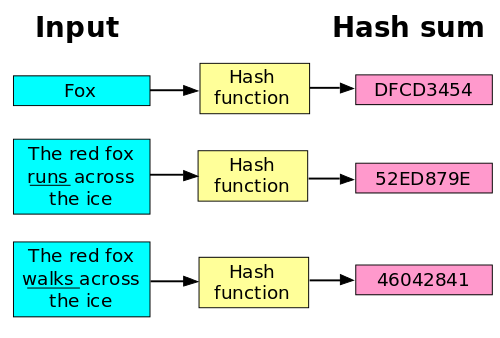
\includegraphics[scale=0.35]{hash_function}
	\caption{TODO citar wiki}
	\label{fig:hash}
\end{figure}

As funções de sentido único tem diversas utilidades na área de computação,
desde na busca de dados em uma estrutura de dados chamado de tabela hash, que
possibilita consultas de forma rápida, até na parte de banco de dados, que é
possível a detecção de registros duplicados ou até mesmo a não integridade de
determinado dado.

Na área de criptografia há ainda a utilização em assinaturas digitais, códigos
de autenticação de mensagens, e ainda outras formas de autenticação. Além do
mais é  muito utilizada em \textit{blockchains}, com sua finalidade em fornecer
prova de trabalho e outras propriedades como utilizar um endereço sem revelar
sua chave pública e consequentemente sua privacidade.

\section{Criptografia homomórfica}

A ideia de usar homomorfismo na criptografia surgiu em um trabalho científico
publicado com o objetivo de propor um criptossistema em um cenário de aumento
da utilização de terminais remotos. Neste caso, não seria ideal ter acesso a
todo o banco de dados cifrados e então decifrá-los para trabalhar os dados.
Neste contexto, surge o conceito de se operar com dados cifrados e obter-se o
mesmo resultado caso se estivesse operando em texto plano.\cite{homomorphic}

Criptografia homomórfica inclui diversos tipos de esquemas de criptografia que
podem ser executados em diferentes classes de dados cifrados. Os tipos mais
comuns de homomorfismo em criptografia são parcialmente homomórfico,
relativamente homomórfico e completamente homomórfico.\cite{survey-homo}

O nome criptografia homomórfica é derivado do conceito de homomorfismo em
álgebra abstrata. Um homomorfismo é uma aplicação que preserva a estrutura
entre duas estruturas algébricas X e Z.

\begin{equation}
f : X \longrightarrow Y
\end{equation}

Seja $\alpha$ uma função de ciframento e $\beta$ uma função de desencriptação
correspondente. Sejam $x1$, $x2$ dados em texto plano. A tupla ($\alpha$,
$\beta$) é uma cifra homomórfica com o operador $\star$ se a propriedade for
satisfeita:

\begin{equation}
\beta (\alpha(x1)) \star (\alpha(x2)) = x1 \star x2
\end{equation}

As operações principais de um esquema homomórfico de criptografia são:
\textit{KeyGen}, \textit{Encryption}, \textit{Decryption}, \textit{Eval}.
\textit{KeyGen} é a operação para criar uma chave pública e outra privada em uma
versão de criptografia assimétrica e a criação de uma chave única em modelo
simétrico. \textit{KeyGen}, \textit{Encryption}, \textit{Decryption} não são
diferentes de suas funções em seus modelos tradicionais.  Entretanto,
\textit{Eval} é uma operação específica de sistemas homomórficos, que tem como
entrada e saída textos cifrados, adicionalmente, o dado cifrado resultante não
deve aumentar de tamanho, caso contrário, haveria um limite de operações
possíveis.\cite{survey-homo}

\begin{figure}[h]
	\centering
	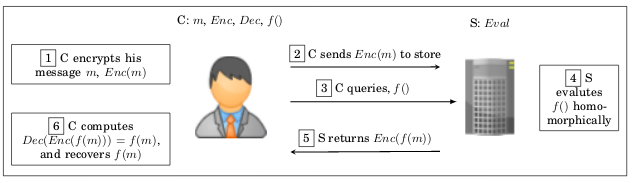
\includegraphics[scale=0.4]{crypto-homo}
	\caption{Imagem tirada do paper ACAR et al., 2018.}
	\label{fig:crypto-homo}
\end{figure}


\section{Blockchain}

Da sua tradução literal, blockchain significa cadeia de blocos. De  maneira
simplista, pode ser definido como um bloco ligado com o anterior, gerando assim
uma cadeia. Estes blocos carregam as informações que são importantes para a
rede. No caso de uma criptomoeda como \textit{Bitcoin}, cada bloco teria dados
sobre as transações realizadas naquele dado instante, ou seja, uma definição do
estado atual do sistema.

A concepção da blockchain foi feita para ser um encadeamento de registros
imutáveis, distribuídos e públicos. Os registros são imutáveis devido ao tipo de
encadeamento que é feito com os blocos, em que o ponteiro para o bloco anterior
é projetado para garantir a imutabilidade dos dados. Como é um protocolo
distribuído, todas as informações não estão armazenadas em um servidor central e
não há um nodo mestre que coordene a rede. Justamente o oposto disso, a
blockchain está replicada em todos os nodos participantes da rede, que podem
estar espalhados pelo mundo inteiro. Além de ser um esquema distribuído, o
referido também é público, pois não há como censurar uma parte de participar da
rede, basta o interessado ter acesso a internet que ele poderá realizar a sua
cópia da base de dados.\cite{blockchain}

\subsection{Cadeia de blocos}

A estrutura de um bloco é basicamente a seguinte:
\begin{itemize}
	\item Constante de valor 0xD9B4BEF9.
	\item Tamanho do bloco em \textit{bytes}.
	\item Cabeçalho do bloco, que consiste em 6 itens.
	\item Quantidade de transações no bloco.
	\item Transações em si.
\end{itemize}

Vale notar que as transações detêm uma estrutura de dados que permite a criação
de \textit{scripts}, além de permitir a inserção de dados arbitrários. \\

Já a estrutura do cabeçalho do bloco é composta por:
\begin{itemize}
	\item Versão do bloco.
	\item \textit{Hash} do bloco anterior.
	\item \textit{Hash} do bloco atual, baseado em todas as transações do bloco.
	\item \textit{Timestamp} em que o bloco foi criado.
	\item \textit{Nonce}, número aleatório que é utilizado na mineração dos blocos.
	\item \textit{Bits}, objetivo atual da mineração em formato compactado.
\end{itemize}

Esta estrutura de dados permite que qualquer participante da rede possa validar
o bloco de maneira rápida. Existe o desafio matemático para a criação de blocos,
isto é, para criar um novo bloco, ele deve calcular um \textit{Hash} com uma
pseudo colisão de acordo com a variável \textit{Bits} do cabeçalho. Resolver
esse desafio matemático é chamado de mineração, e a cada bloco que passa se
torna mais difícil, entretanto, uma vez que sua solução é conhecida, é
extremamente fácil de validar sua corretude. Há diversas soluções possíveis para
determinado bloco, porém é necessário que apenas uma seja
encontrada.\cite{Antonopoulos}

Como a mineração de blocos se torna cada vez mais difícil, a probabilidade de
algum atacante conseguir reescrever um bloco anterior é mínima, visto que ele
teria que concluir o desafio matemático para o bloco que deseja modificar e
ainda todos os sucessores dele.

\begin{figure}[h]
	\centering
	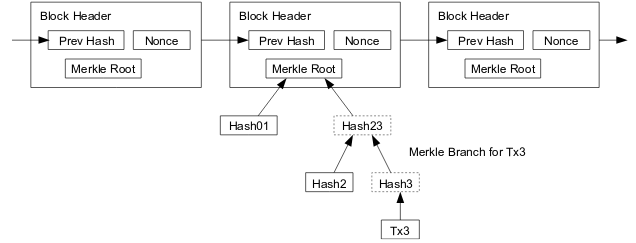
\includegraphics[scale=0.4]{blockchain}
	\caption{Imagem tirada do whitepaper do Bitcoin.}
	\label{fig:blockchain}
\end{figure}

\section{Contratos inteligentes} A ideia de contrato sempre esteve presente
durante todo o curso da humanidade, com a evolução da sociedade foi se criando
novos conceitos para se formalizar uma relação. O contrato é o pilar das
relações econômicas modernas. Entretanto esse mecanismo tem um custo elevado,
durante o processo de criação e utilização de contratos, normalmente baseados em
lei comum, que muitas vezes torna-se inviável para determinados casos.

Idealizado no ano de 1997 por Nick Szabo, os contratos inteligentes foram
pensados como uma substituição natural dos contratos realizados no cotidiano.
Em analogia, a ideia é utilizar de software e hardware para a tomada de
decisões, como em uma máquina automática de vendas de refrigerante. Os
contratos inteligentes vão além da máquina de vendas, uma proposta de
utilização de contratos em todos os tipos de propriedade e controlado do meio
digital. Eles possibilitam a verificação desse contrato de maneira dinâmica e
proativa.\cite{szabo-smart}

Já no surgimento da blockchain descrito no protocolo do Bitcoin, havia espaço
para criação de \textit{scripts} nas transações. Entretanto, estes
\textit{scripts} foram concebidos para serem simples, com a ideia de não
sobrecarregar a rede com a execução de códigos complexos. Um exemplo de
\textit{script} trivial seria o congelamento de fundos até certa data futura.
Como não são  permitido \textit{loops} em sua estrutura, isto impacta na não
Turing completude da linguagem de \textit{script}.\cite{nakamoto2012bitcoin}

Almejando-se ter \textit{scripts} mais potentes, foi criado o conceito de
contratos inteligentes, que são Turing-completos e ainda podem guardar o estado
atual do sistema.  Assim, possibilita a criação de aplicações extremamente mais
complexas.\cite{ethereum}

A \textit{blockchain Ethereum} foi criada juntamente com sua \textit{Virtual
Machine}, a EVM\sigla{EVM}{\emph{Ethereum Virtual Machine}} como é chamada, que
utiliza de um vasto conjunto de instruções para executar tanto tarefas
específicas quanto gerais. Para armazenar os conjuntos de instruções de forma
eficiente, a EVM os codifica em \textit{bytecodes}.\cite{wood2014yellow}

Consequentemente com a criação do conjunto de instruções, houve a criação da uma
linguagem de programação de alto nível que é compilada para esses
\textit{bytecodes} específicos.  \textit{Solidity} foi criada para ser uma
linguagem simples de ser entendida e reproduzida para quem já têm os
conhecimentos de programação de outras linguagens padrões de alto nível.
\cite{solidity}

\begin{figure}[h]
	\centering
	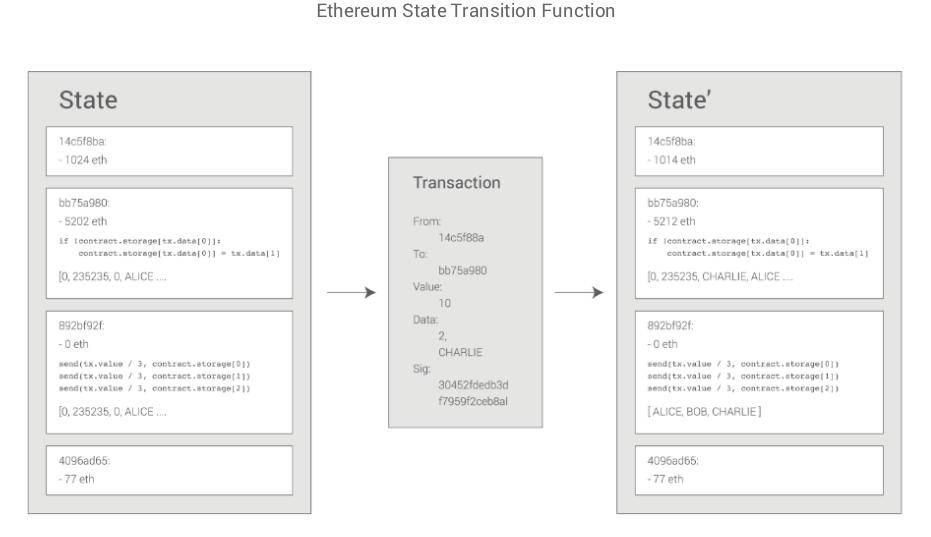
\includegraphics[scale=0.3]{ethereum}
	\caption{Imagem tirada do whitepaper Ethereum}
	\label{fig:ethereum}
\end{figure}

Desta forma, é possível criar aplicações que rodam de forma descentralizada e
que podem ter seu estado atual verificado por qualquer participante do sistema
em qualquer momento além de garantir as propriedades da blockchain.

\chapter{Helios}

Neste capítulo será apresentado o software Helios, em que este trabalho se
baseia para criar um módulo \textit{blockchain} para realizar a prova de
existência das informações importantes dessa uma eleição no Helios.

\chapter{Desenvolvimento}
Este capítulo será abordado a criação do esquema e desenvolvimento do projeto
proposto.

\section{Modificação do software Helios}
Para ter acesso as informações relevantes para o esquema foram criados alguns
\textit{endpoits} que disponibilizam essas informações, sendo essas:

\begin{itemize}
	\item GET `elections/<election\_uuid>/' retorna todas as informações públicas da eleição
	\item GET `elections/<election\_uuid>/voters' retorna todas as informações públicas dos eleitores
	\item GET `elections/<election\_uuid>/result' retorna todas as informações sobre o resultado
\end{itemize}

\section{Contratos inteligentes}

\subsection{Descrição do contrato}

\begin{lstlisting}[language=Solidity]

pragma solidity ^0.5.11;
pragma experimental ABIEncoderV2;

contract Result {
    
    struct Question {
        string question;
        int result;
    }
    
    Question[] public questions;
    string public voters_hash;
    uint256 public relesed_at;
    
    function addQuestion(string memory _question, int _result) public {
        questions.push(Question(_question, _result));
    }
    
    function setVotersHash(string memory _voters_hash) public {
        voters_hash = _voters_hash;
    }
    
    function setReleaseAt(uint256 _relesed_at) public {
        relesed_at = _relesed_at;
    }
}

contract Votes {
    
    struct Vote {
        string vote_hash;
        uint256 cast_at;
    }
    
    Vote[] public votes;
    
    function addVote(string memory _vote_hash, uint256 _cast) public {
        votes.push(Vote(_vote_hash, _cast));
    }
    
}


contract Voters{
    
    struct Voter {
        string uuid;
        string name;
        string email;
    }
    
    Voter[] public voters;
    
    function addVoter(string memory _uuid, string memory _name, string memory _email) public {
        voters.push(Voter(_uuid, _name, _email));
    }
}

contract Election {
    
    string public uuid;
    string public name;
    string public cast_url;
    uint256 public created_at;
    uint256 public voting_starts;
    uint256 public voting_ends;
    
    struct Public_Key {
        string p;
        string q;
        string g;
        string y;
    }
    
    Public_Key public public_key;
    
    struct Question {
        string question;
        string[] anwsers;
    }
    
    Question[] public questions;
    
    Voters public voters_contract;
    Votes public votes_contract;
    Result public result_contract;
    
    constructor(string memory _uuid, string memory _name, string memory _cast_url, uint256 _created_at, uint256 _voting_starts, uint256 _voting_ends,
                string memory _p, string memory _q, string memory _g, string memory _y) public {
        uuid = _uuid;
        name = _name;
        cast_url = _cast_url;
        created_at = _created_at;
        voting_starts = _voting_starts;
        voting_ends = _voting_ends;
        public_key = Public_Key(_p, _q, _g, _y);
        voters_contract = new Voters();
        votes_contract = new Votes();
        result_contract = new Result();
    }
    
    function addQuestion(string memory _question, string[] memory _anwsers) public {
        questions.push(Question(_question, _anwsers));
    }
    
}

\end{lstlisting}

\section{Custo financeiro}

Considerando Gas Price de 25 gwei, visto em 25/09/2019

\begin{table}[]
\centering
\begin{tabular}{|c|c|c|}
\hline
Método        & Gas    & Dólar  \\ \hline
constructor   & 571316 & \$2.41 \\ \hline
addQuestion   & 84624  & \$0.35 \\ \hline
setVotersHash & 87482  & \$0.36 \\ \hline
setReleasedAt & 42164  & \$0.17 \\ \hline
\end{tabular}
\caption{Custos do contrato resultado}
\label{tab:my-table}
\end{table}

\begin{table}[]
\centering
\begin{tabular}{|c|c|c|}
\hline
Método      & Gas    & Dólar  \\ \hline
constructor & 389806 & \$1.64 \\ \hline
addVote     & 128449 & \$0.54 \\ \hline
\end{tabular}
\caption{Custos do contrato votos}
\label{tab:my-table}
\end{table}

\begin{table}[]
\centering
\begin{tabular}{|c|c|c|}
\hline
Método      & Gas    & Dólar  \\ \hline
constructor & 508588 & \$2.14 \\ \hline
addVoter    & 151882 & \$0.64 \\ \hline
\end{tabular}
\caption{Custos do contrato votantes}
\label{tab:my-table}
\end{table}

\begin{table}[]
\centering
\begin{tabular}{|c|c|c|}
\hline
Método      & Gas     & Dólar   \\ \hline
constructor & 2684091 & \$11.34 \\ \hline
addQuestion & 129270  & \$0.54  \\ \hline
\end{tabular}
\caption{Custos do contrato eleição}
\label{tab:my-table}
\end{table}

\chapter{Conclusões}

\section{Trabalhos futuros}

\bibliographystyle{abnt-alf}
\bibliography{ref}


\apendice{}

\chapter{ARTIGO DO TCC}

\end{document}
